%----------------------------------------------------------------------------------------
%	PACKAGES AND OTHER DOCUMENT CONFIGURATIONS
%----------------------------------------------------------------------------------------

\documentclass[a4paper, 11pt]{article} % Font size (can be 10pt, 11pt or 12pt) and paper size (remove a4paper for US letter paper)

\usepackage[protrusion=true,expansion=true]{microtype} % Better typography
\usepackage{graphicx} % Required for including pictures
\usepackage{wrapfig} % Allows in-line images

\usepackage{mathpazo} % Use the Palatino font
\usepackage[T1]{fontenc} % Required for accented characters
\linespread{1.05} % Change line spacing here, Palatino benefits from a slight increase by default

\usepackage{natbib}
\usepackage{attrib}
\usepackage{pgf-pie}

\tolerance=1
\emergencystretch=\maxdimen
\hyphenpenalty=10000
\hbadness=10000

% CUSTOM
\usepackage{url}
\usepackage{subfig}
\usepackage{amsfonts}
\usepackage{booktabs}
\usepackage{siunitx}
\usepackage[toc,page]{appendix}
\usepackage{dcolumn}
\usepackage{rotating}


\makeatletter
\renewcommand\@biblabel[1]{\textbf{#1.}} % Change the square brackets for each bibliography item from '[1]' to '1.'
\renewcommand{\@listI}{\itemsep=0pt} % Reduce the space between items in the itemize and enumerate environments and the bibliography

\renewcommand{\maketitle}{ % Customize the title - do not edit title and author name here, see the TITLE block below
\begin{flushright} % Right align
{\LARGE\@title} % Increase the font size of the title
\vspace{50pt} % Some vertical space between the title and author name

{\large\@author} % Author name
\\\ \today % Date

\vspace{40pt} % Some vertical space between the author block and abstract
\end{flushright}
}

%TC:incbib % Count words

%----------------------------------------------------------------------------------------
%	TITLE
%----------------------------------------------------------------------------------------
%%TC:ignore
\title{\textbf{Analysis of Microdata: Tanzania}\\ % Title
Policy Evaluation and Applied Statistics } % Subtitle

\author{\textsc{Roman Küpper} % Author
\\{\textit{MAS Development and Cooperation NADEL ETHZ 20-22}}} % Institution

\date{\today} % Date

%----------------------------------------------------------------------------------------

%----------------------------------------------------------------------------------------
%	CUSTOM
%----------------------------------------------------------------------------------------
\usepackage{multirow}
\usepackage[colorlinks,citecolor=blue,urlcolor=black,bookmarks=false,hypertexnames=true]{hyperref} 



\begin{document}

\maketitle % Print the title section


%----------------------------------------------------------------------------------------
%	ESSAY BODY
%----------------------------------------------------------------------------------------

\section{Introduction}
% Not sure if i want to keep the subsections in the introduction -> maybe better to merge them in to one
While stunting and mortality for children under five has declined in most countries over the last decades, it is still an important issue in sub-Saharan Africa \cite{Nshimyiryo2019Dec}. It also is and has been an important topic in development where it has been directly mentioned in Goal 4 of the Millennium Development Goals (MDGs) or in several of the Sustainable Development Goals (SDGs). To successfully solve this issue it is vastly important to understand the underlying causes. The following article will therefore analyse data from the Demographic and Health Survey (DHS) for Tanzania to identify country-specific factors that determine if a child is in risk of being stunted or die before the age of five. The study will focus mainly on the effects of per-household income and examine if income is a necessary and sufficient condition for improvements in child health.

\begin{table}[]
  \begin{tabular}{lllll}
  \hline
  \# &  & \textbf{2005} & \textbf{2010} & \textbf{2015} \\ \hline
\textbf{Stunting} & & & &  \\		
no	& 3775 (48.9\%) &	3772 (51.7\%) &	5736 (62.6\%) &	13283 (54.9\%) \\
yes	& 2854 (36.9\%) &	2581 (35.3\%) &	2501 (27.3\%) &	7936 (32.8\%) \\
missing &	1098 (14.2\%) &	950 (13.0\%) &	931 (10.2\%) &	2979 (12.3\%) \\ \hline
\textbf{Under-five mortality} & & & &  \\
no	& 7303 (94.5\%) &	7050 (96.5\%) &	8928 (97.4\%) &	23281 (96.2\%) \\
yes	& 424 (5.5\%) &	253 (3.5\%) &	240 (2.6\%) &	917 (3.8\%) \\ \hline
\textbf{Household income} & & & &  \\						
Mean (SD) &	66.6 (56.5) &	78.0 (60.1) &	82.2 (68.1) &	76.0 (62.5) \\
Median [Min, Max] &	48.2 [6.43, 485] & 60.3 [13.2, 438] & 62.7 [11.2, 426] & 60.3 [6.43, 485] \\ \hline
\textbf{Place of residence} & & & &  \\						
rural &	6383 (82.6\%) &	5918 (81.0\%) &	7034 (76.7\%) &	19335 (79.9\%) \\
urban &	1344 (17.4\%) &	1385 (19.0\%) &	2134 (23.3\%) &	4863 (20.1\%) \\ \hline
\textbf{Mothers age (years)} & & & &  \\						
Mean (SD) &	29.1 (6.80) &	29.7 (6.98) &	29.5 (7.13) & 29.4 (6.99) \\
Median [Min, Max] &	28.0 [15.0, 49.0 &]	29.0 [15.0, 49.0] &	29.0 [15.0, 49.0] &	29.0 [15.0, 49.0] \\ \hline
\textbf{Mothers age (years) at first birth} & & & &  \\						
Mean (SD) &	19.0 (3.10) &	19.2 (3.12) &	19.4 (3.34) & 19.2 (3.20) \\
Median [Min, Max] &	19.0 [10.0, 35.0 &]	19.0 [10.0, 41.0] &	19.0 [10.0, 46.0] &	19.0 [10.0, 46.0] \\ \hline
\textbf{Mothers total children} & & & &  \\						
Mean (SD) &	4.18 (2.55) &	4.26 (2.52) &	4.06 (2.57) & 4.16 (2.55) \\
Median [Min, Max] &	4.00 [1.00, 14.0 &]	4.00 [1.00, 15.0] &	3.00 [1.00, 17.0] &	4.00 [1.00, 17.0] \\ \hline
\textbf{Mothers breastfeeding status} & & & &  \\						
no &	3017 (39.0\%) &	2926 (40.1\%) &	3789 (41.3\%) & 9732 (40.2\%) \\
yes &	4710 (61.0\%) &	4377 (59.9\%) &	5379 (58.7\%) & 14466 (59.8\%) \\ \hline
\textbf{Mother received prenatal care} & & & &  \\						
no &	4230 (54.7\%) &	3344 (45.8\%) &	8705 (94.9\%) & 16279 (67.3\%) \\
yes &	3497 (45.3\%) &	3959 (54.2\%) &	463 (5.1\%) & 7919 (32.7\%) \\ \hline
\textbf{Childs age (months)} & & & &  \\						
Mean (SD) &	28.2 (17.6) &	29.1 (17.6) &	29.0 (17.5) & 28.8 (17.6) \\
Median [Min, Max] &	27.0 [0, 60.0] &	29.0 [0, 60.0] & 28.0 [0, 60.0]	& 28.0 [0, 60.0] \\ \hline
\textbf{Childs sex} & & & &  \\						
male &	3846 (49.8\%) &	3626 (49.7\%) &	4590 (50.1\%) & 12062 (49.8\%) \\
female &	3881 (50.2\%) &	3677 (50.3\%) &	4578 (49.9\%) & 12136 (50.2\%) \\ \hline
\textbf{Water: improved} & & & &  \\						
no &	4048 (52.4\%) &	3822 (52.3\%) &	3999 (43.6\%) & 11869 (49.0\%) \\
yes &	3679 (47.6\%) &	3481 (47.7\%) &	5169 (56.4\%) & 12329 (51.0\%) \\ \hline
\textbf{Sanitation: improved} & & & &  \\						
no &	7328 (94.8\%) &	5841 (80.0\%) &	3068 (33.5\%) & 16237 (67.1\%) \\
yes &	399 (5.2\%) &	1462 (20.0\%) &	6100 (66.5\%) & 7961 (32.9\%) \\ \hline
\textbf{Mother education} & & & &  \\						
noedu &	3390 (43.9\%) &	2986 (40.9\%) &	3208 (35.0\%) & 9584 (39.6\%) \\
primary &	4235 (54.8\%) &	4225 (57.9\%) &	5052 (55.1\%) & 13512 (55.8\%) \\
secondary &	102 (1.3\%) &	92 (1.3\%) &	908 (9.9\%) & 1102 (4.6\%) \\ \hline
\textbf{dead1} & & & &  \\						
no &	1664 (21.5\%) &	1541 (21.1\%) &	1887 (20.6\%) & 5092 (21.0\%) \\
yes &	282 (3.6\%) &	167 (2.3\%) &	144 (1.6\%) & 593 (2.5\%) \\
missing	5781 (74.8\%) &	5595 (76.6\%) &	7137 (77.8\%) & 18513 (76.5\%) \\ \hline
\textbf{dead0} & & & &  \\						
no &	69 (0.9\%) &	68 (0.9\%) &	82 (0.9\%) & 219 (0.9\%) \\
missing &	7658 (99.1\%) &	7235 (99.1\%) &	9086 (99.1\%) & 23979 (99.1\%) \\
&  &  \\ \hline
\end{tabular}
\end{table}

\subsection*{Tanzania}
The situation of Tanzanian children in regard to stunting and under-five mortality has improved over the last three decades. The prevalence for stunting could be decreased from 50\% in the 1990s to 34\% in the year 2015 \cite{UNI18}. The same applies for the under-five mortality rate. The sex-specific under-five mortality rate dropped from 171 to 54 per 1000 births for boys and from 159 to 47 per 1000 births for girls from 1990 to 2019 \cite{UN20}. But despite improvements in recent year, stunting and child mortality in Tanzania are still an ongoing issue in the country. 


\subsection*{Other literature}
Previous research have shown a number of different factors that have an influence on stunting and under-five mortality. Those include the age and sex of the child and various factors concerning the mothers health and education. But also socio-economic factors like the household wealth are mentioned. The factors mentioned in the literature differ for stunting and under-five mortality. Unfinished listings for both, stunting and under-five mortality, can be found in the according tables in Appendix \ref{sec:appendixa} and Appendix \ref{sec:appendixb}.  The tables in the appendix also show how the factors are matched with the variables in our dataset.


\section{Data and Methods}
\subsection*{Sample}

In order to analyse the relationship between income and under-5 mortality and stunting rate a dataset based on the Demographic and Health Surveys (DHS) \cite{DHS20} by ICF International is used. The dataset contains panel data of Tanzanian households for the years 2005, 2010 and 2015. The dataset consists of 24,198 observations for 15,273 households.

\subsection*{Research Strategy}

The aim of this research is to provide a better understanding of the effectiveness of income on under-5-mortality and stunting. For this reason multiple regression models are built to estimate the influence of different independent variables on the two dependent variables (stunting and under-5-mortality). In a first step, only the influence of income on stunting and under-5-mortality IS examined. The formula for the traditional ordinary least squares model (\ref{eqn:simple_regression}) is shown below:

\begin{equation}
 Y_i = \beta_0 + \beta_1 X_i + u_i
 \label{eqn:simple_regression}
\end{equation}

Next, the models are adjusted for survey-year time-fixed effects (\ref{eqn:time_fixed_regression}) with the formula:

\begin{equation}
Y_{it} = \beta_0 + \beta_1 X_{it} + \delta_T BT_t + u_{it}
 \label{eqn:time_fixed_regression}
\end{equation}

The models are then further improved by adding other potentially meaningful variables (\ref{eqn:time_fixed_multiple_regression}) to further reduce the error term. The formula for the multiple regression with regard to time-fixed effects is:

\begin{equation}
Y_{it} = \beta_0 + \beta_1 X_{it} + \delta_2 B2_t + \cdots + \delta_T BT_t + u_{it}
 \label{eqn:time_fixed_multiple_regression}
\end{equation}

Starting from the simple OLS regression the model will be further enhanced by including additional variables and time fixed effects. 

\subsection*{Variables}
- Binary outcome variables (stunting \& dead5)\\
- Main explanatory variable (log\_y)

\subsection*{Dataset / Descriptive Statistics}

\begin{figure}[h!]
    \centering
    \subfloat[\centering dead5 over time]{{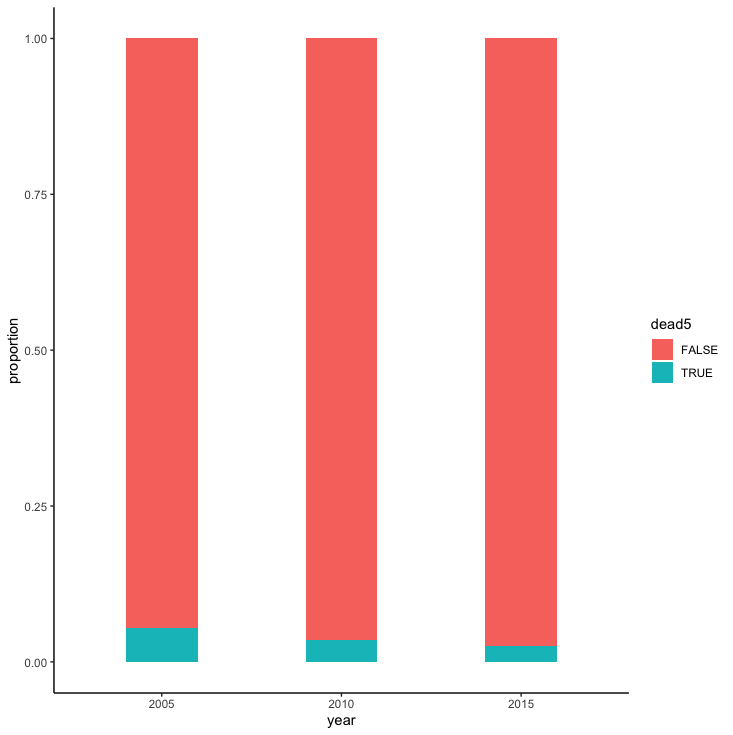
\includegraphics[width=5cm]{figures/dead5_proportion} }}%
    \qquad
    \subfloat[\centering stunting over time]{{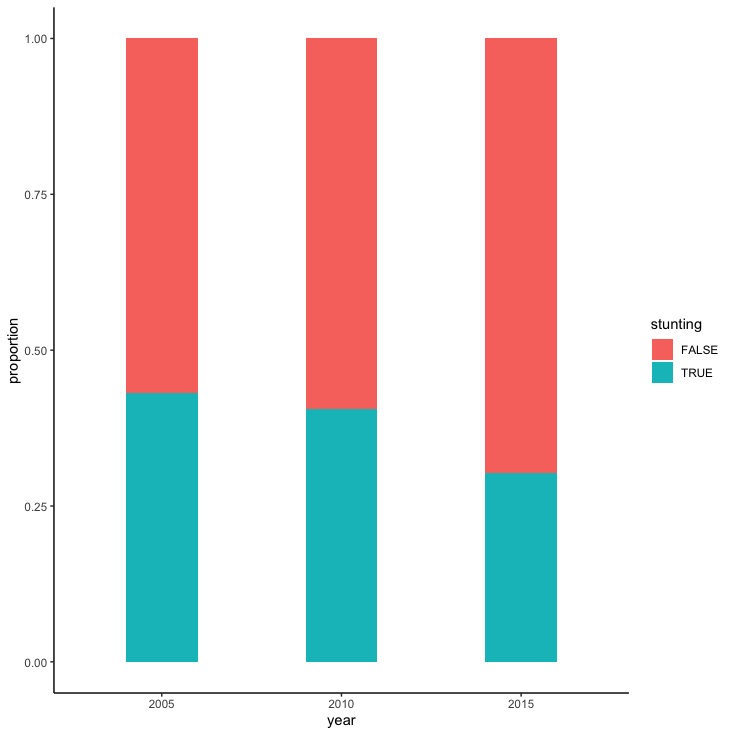
\includegraphics[width=5cm]{figures/stunting_proportion} }}%
    \caption{Stunting and Under-5-Mortality over time}%
    \label{fig:stunting_dead5_proportion}%
\end{figure}

\begin{figure}[h!]
    \centering
    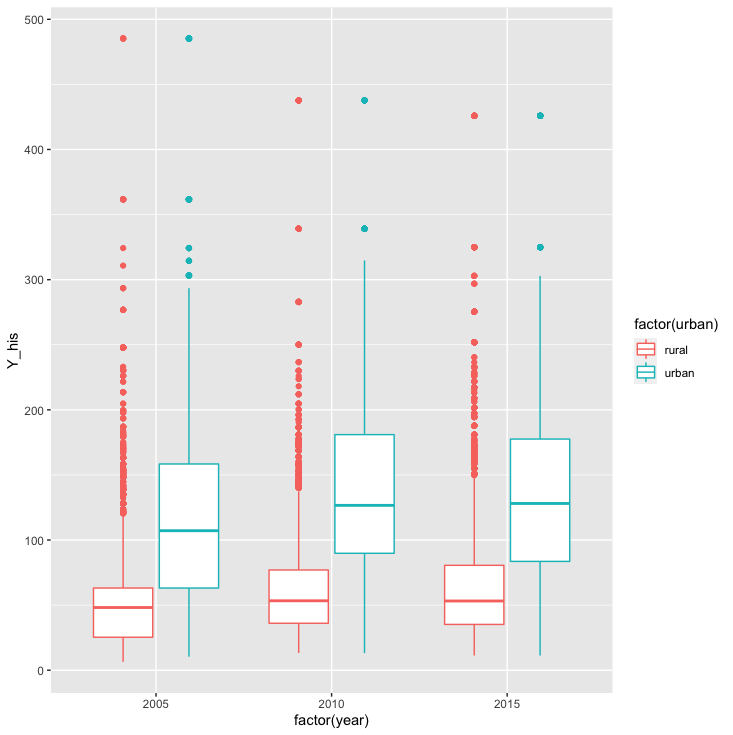
\includegraphics[scale=0.4]{figures/income_over_time} 
    \caption{Y\_his over time}
    \label{fig:income_over_time}
\end{figure}


\begin{figure}[h!]
    \centering
    \subfloat[\centering water situation over time]{{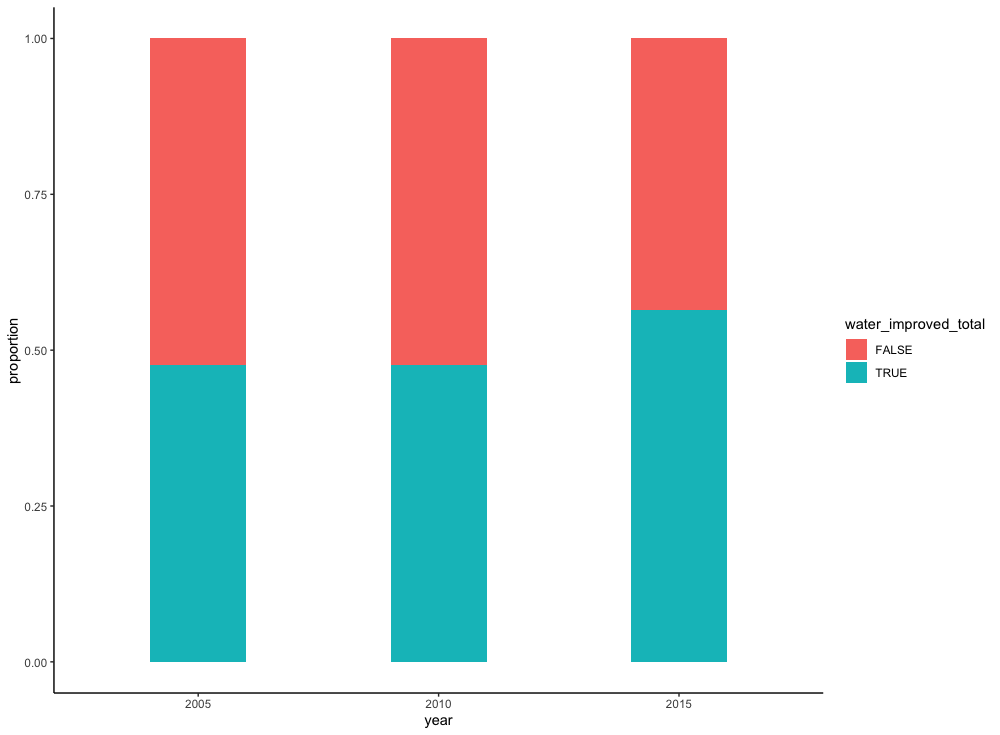
\includegraphics[width=5cm]{figures/water_improved_proportion} }}%
    \qquad
    \subfloat[\centering sanitation over time]{{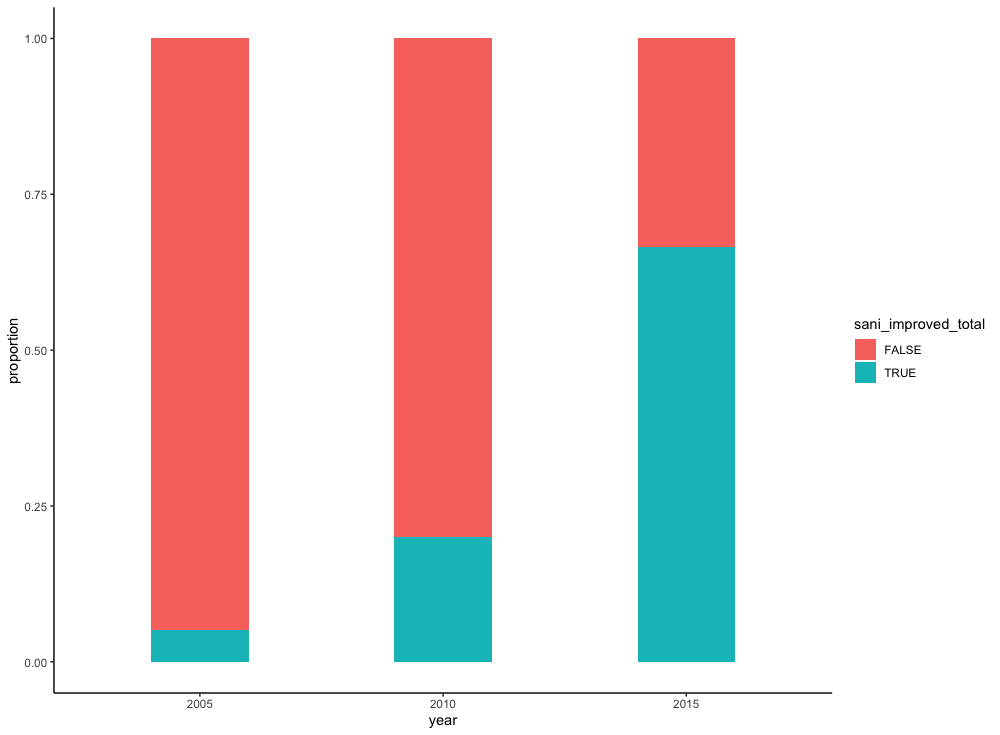
\includegraphics[width=5cm]{figures/sanitation_improved_proportion} }}%
    \caption{Water and Sanitation over time}%
    \label{fig:water_sanitation_proportion}%
\end{figure}


Another often quoted factor for the well-being of children is their mothers education. The dataset include information on three different variables for education. Namely primary, secondary and no education. The interpretation of the data is somewhat difficult. Some of the observations have specify that a mother has both primary and no education at the same time. When this data is interpreted as "the mother has started but not finished her primary education", the corresponding barplot is shown in figure (\ref{fig:education_proportion})(a). 

\begin{figure}[h!]
    \centering
    \subfloat[\centering highest education over time]{{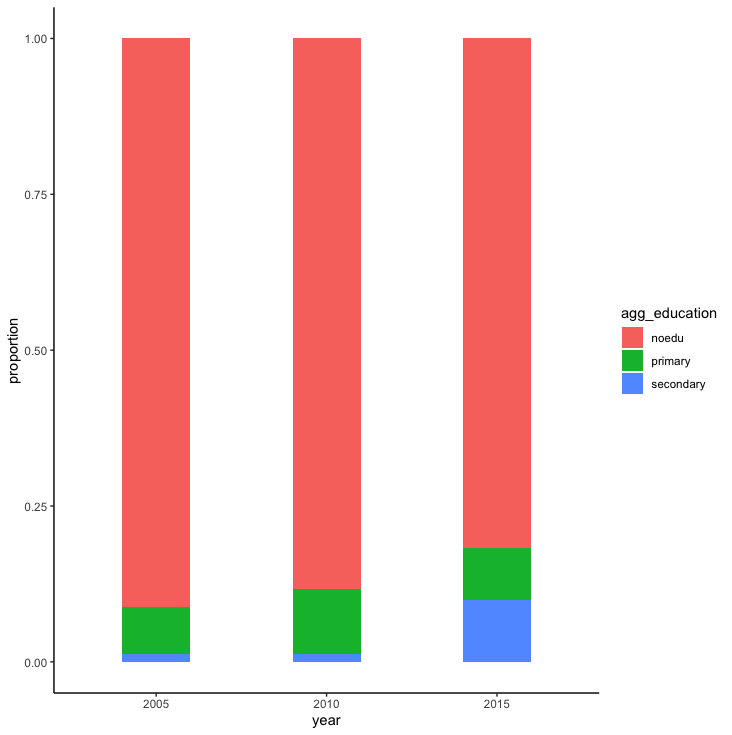
\includegraphics[width=5cm]{figures/aggregated_education_indoubt_lower} }}%
    \qquad
    \subfloat[\centering highest education over time]{{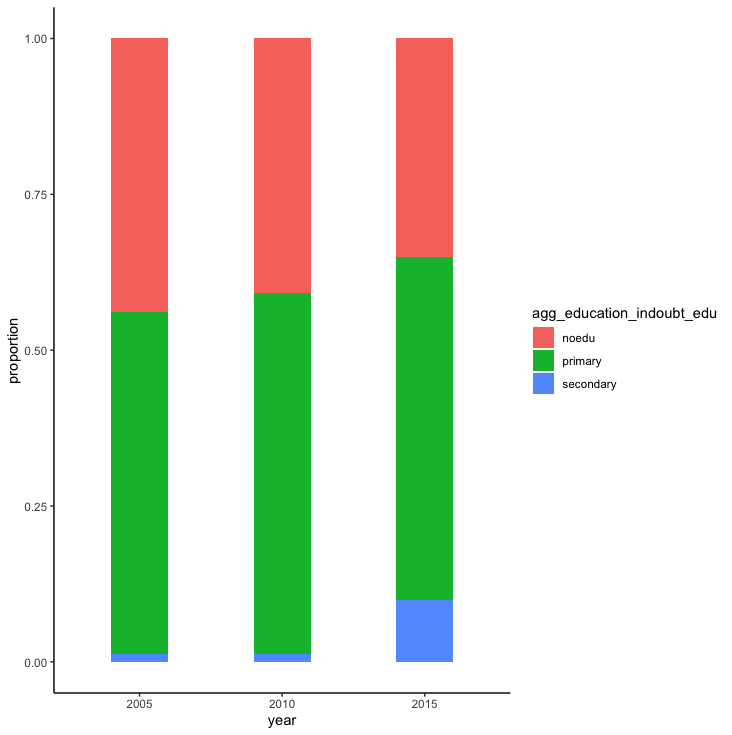
\includegraphics[width=5cm]{figures/aggregated_education_indoubt_higher} }}%
    \caption{Highest education over time - aggregated}%
    \label{fig:education_proportion}%
\end{figure}

But when looking at other studies \cite{SAM08} on the distribution of primary, secondary on no-education in Tanzania, the share of uneducated women seems to be too high. If the ambiguous values are interpreted as "the education is not finished yet, but will be"\footnote{When an observation has "mo\_noedu == 1" and "mo\_primary== 1" the variables are aggregated to  to "education = primary".}, our data is more in line with other studies. The graphic representation of this can be found in figure (\ref{fig:education_proportion})(b).  


\begin{sidewaystable}[!htbp] \centering 
  \caption{Regressions Using Demographic and Health Surveys} 
  \label{} 
  \scalebox{0.75}{
\begin{tabular}{@{\extracolsep{5pt}}lD{.}{.}{-5} D{.}{.}{-5} D{.}{.}{-5} D{.}{.}{-5} D{.}{.}{-5} D{.}{.}{-5} } 
\\[-1.8ex]\hline 
\hline \\[-1.8ex] 
 & \multicolumn{6}{c}{\textit{Dependent variable:}} \\ 
\cline{2-7} 
\\[-1.8ex] & \multicolumn{3}{c}{stunting} & \multicolumn{3}{c}{dead5} \\ 
 & \multicolumn{1}{c}{(I)} & \multicolumn{1}{c}{(II)} & \multicolumn{1}{c}{(III)} & \multicolumn{1}{c}{(IV)} & \multicolumn{1}{c}{(V)} & \multicolumn{1}{c}{(VI)} \\ 
\\[-1.8ex] & \multicolumn{1}{c}{} & \multicolumn{1}{c}{NA} & \multicolumn{1}{c}{NA} & \multicolumn{1}{c}{NA} & \multicolumn{1}{c}{NA} & \multicolumn{1}{c}{NA}\\ 
\hline \\[-1.8ex] 
 log\_y & -0.10287^{***} & -0.09724^{***} & -0.06086^{***} & -0.00832^{***} & -0.00632^{***} & -0.00353 \\ 
  & (0.00431) & (0.00433) & (0.00578) & (0.00162) & (0.00161) & (0.00222) \\ 
  as.factor(urban)urban &  &  & -0.04084^{***} &  &  & 0.00568^{*} \\ 
  &  &  & (0.00891) &  &  & (0.00341) \\ 
  c\_age &  &  & 0.00287^{***} &  &  &  \\ 
  &  &  & (0.00020) &  &  &  \\ 
  c\_sex &  &  & -0.05035^{***} &  &  & -0.00095 \\ 
  &  &  & (0.00645) &  &  & (0.00244) \\ 
  c\_first &  &  &  &  &  & 0.02076^{***} \\ 
  &  &  &  &  &  & (0.00370) \\ 
  mo\_assistance &  &  &  &  &  & -0.00631^{**} \\ 
  &  &  &  &  &  & (0.00314) \\ 
  mo\_breastfeeedingyes &  &  &  &  &  & -0.02894^{***} \\ 
  &  &  &  &  &  & (0.00267) \\ 
  mo\_age\_birth &  &  & -0.00142^{***} &  &  & 0.00180^{***} \\ 
  &  &  & (0.00048) &  &  & (0.00023) \\ 
  as.factor(mo\_breastfeeeding)yes &  &  & -0.04470^{***} &  &  &  \\ 
  &  &  & (0.00756) &  &  &  \\ 
  mo\_noedu &  &  & 0.06406^{***} &  &  &  \\ 
  &  &  & (0.01163) &  &  &  \\ 
  mo\_primary &  &  & -0.02500^{***} &  &  & -0.00395 \\ 
  &  &  & (0.00724) &  &  & (0.00272) \\ 
  mo\_secondary &  &  & -0.02048 &  &  & -0.01305^{***} \\ 
  &  &  & (0.01592) &  &  & (0.00442) \\ 
  water\_improved\_total &  &  & -0.02182^{***} &  &  & -0.00982^{***} \\ 
  &  &  & (0.00710) &  &  & (0.00273) \\ 
  sani\_improved\_total &  &  & -0.01866^{**} &  &  & -0.00636^{**} \\ 
  &  &  & (0.00908) &  &  & (0.00317) \\ 
  Constant & 0.79150^{***} & 0.81154^{***} & 0.70546^{***} & 0.07170^{***} & 0.07966^{***} & 0.04437^{***} \\ 
  & (0.01817) & (0.01828) & (0.03274) & (0.00689) & (0.00710) & (0.01115) \\ 
 \hline \\[-1.8ex] 
Observations & \multicolumn{1}{c}{21,219} & \multicolumn{1}{c}{21,219} & \multicolumn{1}{c}{21,219} & \multicolumn{1}{c}{24,198} & \multicolumn{1}{c}{24,198} & \multicolumn{1}{c}{24,198} \\ 
R$^{2}$ & \multicolumn{1}{c}{0.02397} & \multicolumn{1}{c}{0.03486} & \multicolumn{1}{c}{0.05976} & \multicolumn{1}{c}{0.00102} & \multicolumn{1}{c}{0.00462} & \multicolumn{1}{c}{0.01457} \\ 
Adjusted R$^{2}$ & \multicolumn{1}{c}{0.02392} & \multicolumn{1}{c}{0.03472} & \multicolumn{1}{c}{0.05919} & \multicolumn{1}{c}{0.00098} & \multicolumn{1}{c}{0.00449} & \multicolumn{1}{c}{0.01404} \\ 
\hline 
\hline \\[-1.8ex] 
\textit{Note:}  & \multicolumn{6}{r}{$^{*}$p$<$0.1; $^{**}$p$<$0.05; $^{***}$p$<$0.01} \\ 
\end{tabular} 
}
\end{sidewaystable}


%----------------------------------------------------------------------------------------
% BIBLIOGRAPHY
%----------------------------------------------------------------------------------------
\newpage
\bibliographystyle{plain}
\bibliography{main.bib}

%----------------------------------------------------------------------------------------

%----------------------------------------------------------------------------------------
% APPENDIX
%----------------------------------------------------------------------------------------
\newpage
\begin{appendices}
\section{Factors and variables for stunting} \label{sec:appendixa}
\begin{table}[h!]
\begin{tabular}{@{}lll@{}}
\toprule
\# & \textbf{Factors} & \textbf{Corresponding variable} \\ \midrule
1 & Childs age & c\_age \\
2 & Sex of child & c\_sex  \\
3 & Birth weight & -  \\
4 & Birth size & - \\ \midrule

5 & Mothers health & - \\
6 & Mothers education & mo\_noedu, mo\_primary, mo\_secondary \\
7 & Mothers age  & mo\_age\_birth \\
8 & Mothers BMI & - \\
9 & Breastfeeding & mo\_breastfeeding \\ \midrule

10 & Wealth of household & Y\_his  \\
11 & Social inequality & income\_quintile \\
12 & Source of drinking water & water\_improved\_total  \\
13 & Sanitation &  sani\_improved\_total  \\
14 & Place of residence & urban  \\ \bottomrule
\end{tabular}
    \caption{Factors associated with childhood stunting, wasting and underweight. Sources: \cite{Akombi2017Aug} \cite{UNI18}}
    \label{table:stunting}
\end{table}

\newpage
\section{Factors and variables for under-five mortality} \label{sec:appendixb}
\begin{table}[h!]
\begin{tabular}{@{}lll@{}}
\toprule
\# & \textbf{Factors} & \textbf{Corresponding variable} \\ \midrule
1 & Sex of child & c\_sex  \\
2 & Birth order & c\_first  \\ 
3 & Malnutrition & - \\ 
4 & Vaccinations & - \\ \midrule

5 & Access to postnatal care & mo\_assistance \\
6 & Mothers age & mo\_age\_birth \\
7 & Education & mo\_noedu, mo\_primary, mo\_secondary \\
8 & Breastfeeding & mo\_breastfeeding \\
9 & Place of delivery & - \\ \midrule

10 & Household wealth & Y\_his \\
11 & Place of residence  & urban \\ 
12 & Source of drinking water & water\_improved\_total  \\
13 & Sanitation &  sani\_improved\_total  \\ \bottomrule
\end{tabular}
    \caption{Factors associated with under-five mortality. Sources: \cite{Ettarh2012Mar}\cite{Who2020Sep}} \cite{UNICEF2006}
    \label{table:dead5}
\end{table}


\newpage
\section{Correlation-matrix for stunting} \label{sec:appendixc}
\begin{figure}[h!]
    \centering
    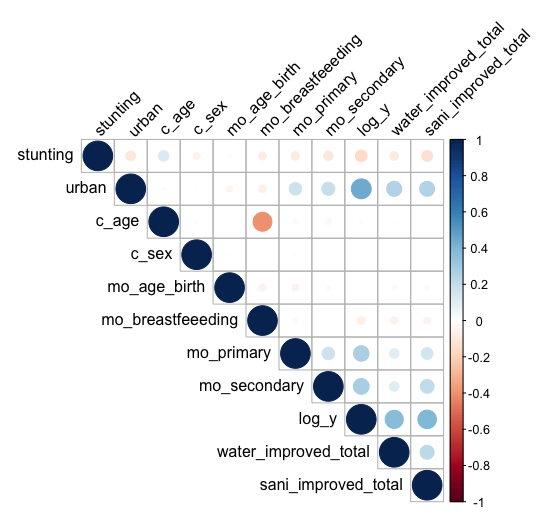
\includegraphics[scale=0.6]{figures/corrmatrix_stunting} 
    \caption{Correlation-matrix that should help to find variables that have a significant effect on stunting.}
    \label{fig:corrmatrix_stunting}
\end{figure}


\newpage
\section{Correlation-matrix for under-five mortality} \label{sec:appendixd}
\begin{figure}[h!]
    \centering
    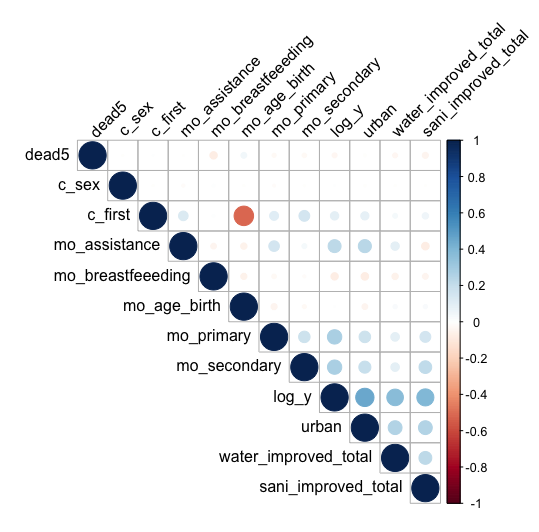
\includegraphics[scale=0.6]{figures/corrmatrix_dead5} 
    \caption{Correlation-matrix that should help to find variables that have a significant effect on under-five mortality.}
    \label{fig:corrmatrix_dead5}
\end{figure}

\end{appendices}
%----------------------------------------------------------------------------------------

\end{document}